\documentclass[1p]{elsarticle_modified}
%\bibliographystyle{elsarticle-num}

%\usepackage[colorlinks]{hyperref}
%\usepackage{abbrmath_seonhwa} %\Abb, \Ascr, \Acal ,\Abf, \Afrak
\usepackage{amsfonts}
\usepackage{amssymb}
\usepackage{amsmath}
\usepackage{amsthm}
\usepackage{scalefnt}
\usepackage{amsbsy}
\usepackage{kotex}
\usepackage{caption}
\usepackage{subfig}
\usepackage{color}
\usepackage{graphicx}
\usepackage{xcolor} %% white, black, red, green, blue, cyan, magenta, yellow
\usepackage{float}
\usepackage{setspace}
\usepackage{hyperref}

\usepackage{tikz}
\usetikzlibrary{arrows}

\usepackage{multirow}
\usepackage{array} % fixed length table
\usepackage{hhline}

%%%%%%%%%%%%%%%%%%%%%
\makeatletter
\renewcommand*\env@matrix[1][\arraystretch]{%
	\edef\arraystretch{#1}%
	\hskip -\arraycolsep
	\let\@ifnextchar\new@ifnextchar
	\array{*\c@MaxMatrixCols c}}
\makeatother %https://tex.stackexchange.com/questions/14071/how-can-i-increase-the-line-spacing-in-a-matrix
%%%%%%%%%%%%%%%

\usepackage[normalem]{ulem}

\newcommand{\msout}[1]{\ifmmode\text{\sout{\ensuremath{#1}}}\else\sout{#1}\fi}
%SOURCE: \msout is \stkout macro in https://tex.stackexchange.com/questions/20609/strikeout-in-math-mode

\newcommand{\cancel}[1]{
	\ifmmode
	{\color{red}\msout{#1}}
	\else
	{\color{red}\sout{#1}}
	\fi
}

\newcommand{\add}[1]{
	{\color{blue}\uwave{#1}}
}

\newcommand{\replace}[2]{
	\ifmmode
	{\color{red}\msout{#1}}{\color{blue}\uwave{#2}}
	\else
	{\color{red}\sout{#1}}{\color{blue}\uwave{#2}}
	\fi
}

\newcommand{\Sol}{\mathcal{S}} %segment
\newcommand{\D}{D} %diagram
\newcommand{\A}{\mathcal{A}} %arc


%%%%%%%%%%%%%%%%%%%%%%%%%%%%%5 test

\def\sl{\operatorname{\textup{SL}}(2,\Cbb)}
\def\psl{\operatorname{\textup{PSL}}(2,\Cbb)}
\def\quan{\mkern 1mu \triangleright \mkern 1mu}

\theoremstyle{definition}
\newtheorem{thm}{Theorem}[section]
\newtheorem{prop}[thm]{Proposition}
\newtheorem{lem}[thm]{Lemma}
\newtheorem{ques}[thm]{Question}
\newtheorem{cor}[thm]{Corollary}
\newtheorem{defn}[thm]{Definition}
\newtheorem{exam}[thm]{Example}
\newtheorem{rmk}[thm]{Remark}
\newtheorem{alg}[thm]{Algorithm}

\newcommand{\I}{\sqrt{-1}}
\begin{document}

%\begin{frontmatter}
%
%\title{Boundary parabolic representations of knots up to 8 crossings}
%
%%% Group authors per affiliation:
%\author{Yunhi Cho} 
%\address{Department of Mathematics, University of Seoul, Seoul, Korea}
%\ead{yhcho@uos.ac.kr}
%
%
%\author{Seonhwa Kim} %\fnref{s_kim}}
%\address{Center for Geometry and Physics, Institute for Basic Science, Pohang, 37673, Korea}
%\ead{ryeona17@ibs.re.kr}
%
%\author{Hyuk Kim}
%\address{Department of Mathematical Sciences, Seoul National University, Seoul 08826, Korea}
%\ead{hyukkim@snu.ac.kr}
%
%\author{Seokbeom Yoon}
%\address{Department of Mathematical Sciences, Seoul National University, Seoul, 08826,  Korea}
%\ead{sbyoon15@snu.ac.kr}
%
%\begin{abstract}
%We find all boundary parabolic representation of knots up to 8 crossings.
%
%\end{abstract}
%\begin{keyword}
%    \MSC[2010] 57M25 
%\end{keyword}
%
%\end{frontmatter}

%\linenumbers
%\tableofcontents
%
\newcommand\colored[1]{\textcolor{white}{\rule[-0.35ex]{0.8em}{1.4ex}}\kern-0.8em\color{red} #1}%
%\newcommand\colored[1]{\textcolor{white}{ #1}\kern-2.17ex	\textcolor{white}{ #1}\kern-1.81ex	\textcolor{white}{ #1}\kern-2.15ex\color{red}#1	}

{\Large $\underline{12a_{0470}~(K12a_{0470})}$}

\setlength{\tabcolsep}{10pt}
\renewcommand{\arraystretch}{1.6}
\vspace{1cm}\begin{tabular}{m{100pt}>{\centering\arraybackslash}m{274pt}}
\multirow{5}{120pt}{
	\centering
	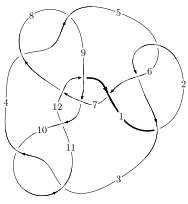
\includegraphics[width=112pt]{../../../GIT/diagram.site/Diagrams/png/1271_12a_0470.png}\\
\ \ \ A knot diagram\footnotemark}&
\allowdisplaybreaks
\textbf{Linearized knot diagam} \\
\cline{2-2}
 &
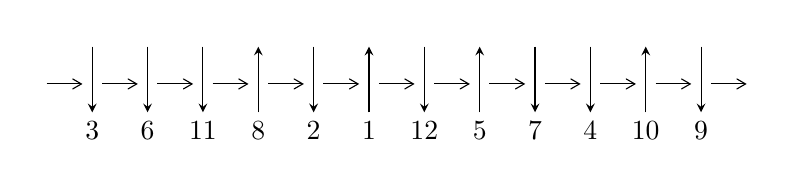
\begin{tikzpicture}[x=20pt, y=17pt]
	% nodes
	\node (C0) at (0, 0) {};
	\node (C1) at (1, 0) {};
	\node (C1U) at (1, +1) {};
	\node (C1D) at (1, -1) {3};

	\node (C2) at (2, 0) {};
	\node (C2U) at (2, +1) {};
	\node (C2D) at (2, -1) {6};

	\node (C3) at (3, 0) {};
	\node (C3U) at (3, +1) {};
	\node (C3D) at (3, -1) {11};

	\node (C4) at (4, 0) {};
	\node (C4U) at (4, +1) {};
	\node (C4D) at (4, -1) {8};

	\node (C5) at (5, 0) {};
	\node (C5U) at (5, +1) {};
	\node (C5D) at (5, -1) {2};

	\node (C6) at (6, 0) {};
	\node (C6U) at (6, +1) {};
	\node (C6D) at (6, -1) {1};

	\node (C7) at (7, 0) {};
	\node (C7U) at (7, +1) {};
	\node (C7D) at (7, -1) {12};

	\node (C8) at (8, 0) {};
	\node (C8U) at (8, +1) {};
	\node (C8D) at (8, -1) {5};

	\node (C9) at (9, 0) {};
	\node (C9U) at (9, +1) {};
	\node (C9D) at (9, -1) {7};

	\node (C10) at (10, 0) {};
	\node (C10U) at (10, +1) {};
	\node (C10D) at (10, -1) {4};

	\node (C11) at (11, 0) {};
	\node (C11U) at (11, +1) {};
	\node (C11D) at (11, -1) {10};

	\node (C12) at (12, 0) {};
	\node (C12U) at (12, +1) {};
	\node (C12D) at (12, -1) {9};
	\node (C13) at (13, 0) {};

	% arrows
	\draw[->,>={angle 60}]
	(C0) edge (C1) (C1) edge (C2) (C2) edge (C3) (C3) edge (C4) (C4) edge (C5) (C5) edge (C6) (C6) edge (C7) (C7) edge (C8) (C8) edge (C9) (C9) edge (C10) (C10) edge (C11) (C11) edge (C12) (C12) edge (C13) ;	\draw[->,>=stealth]
	(C1U) edge (C1D) (C2U) edge (C2D) (C3U) edge (C3D) (C4D) edge (C4U) (C5U) edge (C5D) (C6D) edge (C6U) (C7U) edge (C7D) (C8D) edge (C8U) (C9U) edge (C9D) (C10U) edge (C10D) (C11D) edge (C11U) (C12U) edge (C12D) ;
	\end{tikzpicture} \\
\hhline{~~} \\& 
\textbf{Solving Sequence} \\ \cline{2-2} 
 &
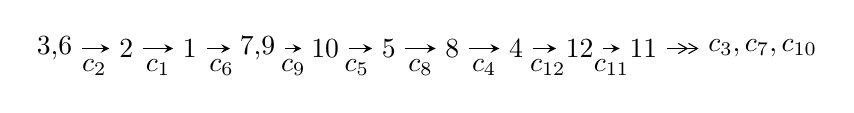
\begin{tikzpicture}[x=23pt, y=7pt]
	% node
	\node (A0) at (-1/8, 0) {3,6};
	\node (A1) at (1, 0) {2};
	\node (A2) at (2, 0) {1};
	\node (A3) at (49/16, 0) {7,9};
	\node (A4) at (33/8, 0) {10};
	\node (A5) at (41/8, 0) {5};
	\node (A6) at (49/8, 0) {8};
	\node (A7) at (57/8, 0) {4};
	\node (A8) at (65/8, 0) {12};
	\node (A9) at (73/8, 0) {11};
	\node (C1) at (1/2, -1) {$c_{2}$};
	\node (C2) at (3/2, -1) {$c_{1}$};
	\node (C3) at (5/2, -1) {$c_{6}$};
	\node (C4) at (29/8, -1) {$c_{9}$};
	\node (C5) at (37/8, -1) {$c_{5}$};
	\node (C6) at (45/8, -1) {$c_{8}$};
	\node (C7) at (53/8, -1) {$c_{4}$};
	\node (C8) at (61/8, -1) {$c_{12}$};
	\node (C9) at (69/8, -1) {$c_{11}$};
	\node (A10) at (11, 0) {$c_{3},c_{7},c_{10}$};

	% edge
	\draw[->,>=stealth]	
	(A0) edge (A1) (A1) edge (A2) (A2) edge (A3) (A3) edge (A4) (A4) edge (A5) (A5) edge (A6) (A6) edge (A7) (A7) edge (A8) (A8) edge (A9) ;
	\draw[->>,>={angle 60}]	
	(A9) edge (A10);
\end{tikzpicture} \\ 

\end{tabular} \\

\footnotetext{
The image of knot diagram is generated by the software ``\textbf{Draw programme}" developed by Andrew Bartholomew(\url{http://www.layer8.co.uk/maths/draw/index.htm\#Running-draw}), where we modified some parts for our purpose(\url{https://github.com/CATsTAILs/LinksPainter}).
}\phantom \\ \newline 
\centering \textbf{Ideals for irreducible components\footnotemark of $X_{\text{par}}$} 
 
\begin{align*}
I^u_{1}&=\langle 
4.04726\times10^{246} u^{151}-6.41758\times10^{246} u^{150}+\cdots+5.27327\times10^{246} b+2.97396\times10^{246},\\
\phantom{I^u_{1}}&\phantom{= \langle  }7.15742\times10^{246} u^{151}-9.25761\times10^{246} u^{150}+\cdots+5.27327\times10^{246} a-1.31606\times10^{247},\;u^{152}-2 u^{151}+\cdots+u-1\rangle \\
I^u_{2}&=\langle 
8 u^{28}+4 u^{27}+\cdots+b-8,\;5 u^{28}+6 u^{27}+\cdots+a-5,\;u^{29}+u^{28}+\cdots- u-1\rangle \\
\\
\end{align*}
\raggedright * 2 irreducible components of $\dim_{\mathbb{C}}=0$, with total 181 representations.\\
\footnotetext{All coefficients of polynomials are rational numbers. But the coefficients are sometimes approximated in decimal forms when there is not enough margin.}
\newpage
\renewcommand{\arraystretch}{1}
\centering \section*{I. $I^u_{1}= \langle 4.05\times10^{246} u^{151}-6.42\times10^{246} u^{150}+\cdots+5.27\times10^{246} b+2.97\times10^{246},\;7.16\times10^{246} u^{151}-9.26\times10^{246} u^{150}+\cdots+5.27\times10^{246} a-1.32\times10^{247},\;u^{152}-2 u^{151}+\cdots+u-1 \rangle$}
\flushleft \textbf{(i) Arc colorings}\\
\begin{tabular}{m{7pt} m{180pt} m{7pt} m{180pt} }
\flushright $a_{3}=$&$\begin{pmatrix}1\\0\end{pmatrix}$ \\
\flushright $a_{6}=$&$\begin{pmatrix}0\\u\end{pmatrix}$ \\
\flushright $a_{2}=$&$\begin{pmatrix}1\\- u^2\end{pmatrix}$ \\
\flushright $a_{1}=$&$\begin{pmatrix}- u^2+1\\- u^2\end{pmatrix}$ \\
\flushright $a_{7}=$&$\begin{pmatrix}u^5-2 u^3+u\\u^5- u^3+u\end{pmatrix}$ \\
\flushright $a_{9}=$&$\begin{pmatrix}-1.35730 u^{151}+1.75558 u^{150}+\cdots-5.13107 u+2.49572\\-0.767505 u^{151}+1.21700 u^{150}+\cdots-0.938204 u-0.563969\end{pmatrix}$ \\
\flushright $a_{10}=$&$\begin{pmatrix}-1.24710 u^{151}+2.18343 u^{150}+\cdots-5.16086 u+3.31368\\-1.61120 u^{151}+2.24775 u^{150}+\cdots-0.307596 u-1.05852\end{pmatrix}$ \\
\flushright $a_{5}=$&$\begin{pmatrix}u\\- u^3+u\end{pmatrix}$ \\
\flushright $a_{8}=$&$\begin{pmatrix}-1.64848 u^{151}+2.79384 u^{150}+\cdots-5.42734 u+2.23244\\-1.90549 u^{151}+2.80402 u^{150}+\cdots-0.487392 u-1.28317\end{pmatrix}$ \\
\flushright $a_{4}=$&$\begin{pmatrix}-1.00094 u^{151}+3.31075 u^{150}+\cdots-4.77710 u-2.74348\\0.190513 u^{151}-1.42765 u^{150}+\cdots-2.05798 u+1.60425\end{pmatrix}$ \\
\flushright $a_{12}=$&$\begin{pmatrix}3.78395 u^{151}-7.66715 u^{150}+\cdots+9.27456 u-1.33763\\0.377582 u^{151}-1.13512 u^{150}+\cdots+5.43079 u-1.54915\end{pmatrix}$ \\
\flushright $a_{11}=$&$\begin{pmatrix}7.65369 u^{151}-11.9415 u^{150}+\cdots-5.79642 u+3.51479\\0.585467 u^{151}-0.0463453 u^{150}+\cdots-0.251655 u+1.47548\end{pmatrix}$\\&\end{tabular}
\flushleft \textbf{(ii) Obstruction class $= -1$}\\~\\
\flushleft \textbf{(iii) Cusp Shapes $= -0.0982650 u^{151}-5.31022 u^{150}+\cdots+12.0206 u-0.0299219$}\\~\\
\newpage\renewcommand{\arraystretch}{1}
\flushleft \textbf{(iv) u-Polynomials at the component}\newline \\
\begin{tabular}{m{50pt}|m{274pt}}
Crossings & \hspace{64pt}u-Polynomials at each crossing \\
\hline $$\begin{aligned}c_{1}\end{aligned}$$&$\begin{aligned}
&u^{152}+76 u^{151}+\cdots+13 u+1
\end{aligned}$\\
\hline $$\begin{aligned}c_{2},c_{5}\end{aligned}$$&$\begin{aligned}
&u^{152}+2 u^{151}+\cdots- u-1
\end{aligned}$\\
\hline $$\begin{aligned}c_{3},c_{10}\end{aligned}$$&$\begin{aligned}
&u^{152}+33 u^{150}+\cdots+783 u+259
\end{aligned}$\\
\hline $$\begin{aligned}c_{4},c_{8}\end{aligned}$$&$\begin{aligned}
&u^{152}+u^{151}+\cdots+6 u+1
\end{aligned}$\\
\hline $$\begin{aligned}c_{6}\end{aligned}$$&$\begin{aligned}
&u^{152}+6 u^{151}+\cdots-3317745 u-609725
\end{aligned}$\\
\hline $$\begin{aligned}c_{7}\end{aligned}$$&$\begin{aligned}
&u^{152}- u^{151}+\cdots+57 u-1
\end{aligned}$\\
\hline $$\begin{aligned}c_{9}\end{aligned}$$&$\begin{aligned}
&u^{152}-20 u^{151}+\cdots+21337 u-12353
\end{aligned}$\\
\hline $$\begin{aligned}c_{11}\end{aligned}$$&$\begin{aligned}
&u^{152}-66 u^{151}+\cdots-1636585 u+67081
\end{aligned}$\\
\hline $$\begin{aligned}c_{12}\end{aligned}$$&$\begin{aligned}
&u^{152}-14 u^{151}+\cdots-30 u+1
\end{aligned}$\\
\hline
\end{tabular}\\~\\
\newpage\renewcommand{\arraystretch}{1}
\flushleft \textbf{(v) Riley Polynomials at the component}\newline \\
\begin{tabular}{m{50pt}|m{274pt}}
Crossings & \hspace{64pt}Riley Polynomials at each crossing \\
\hline $$\begin{aligned}c_{1}\end{aligned}$$&$\begin{aligned}
&y^{152}+4 y^{151}+\cdots-105 y+1
\end{aligned}$\\
\hline $$\begin{aligned}c_{2},c_{5}\end{aligned}$$&$\begin{aligned}
&y^{152}-76 y^{151}+\cdots-13 y+1
\end{aligned}$\\
\hline $$\begin{aligned}c_{3},c_{10}\end{aligned}$$&$\begin{aligned}
&y^{152}+66 y^{151}+\cdots+1636585 y+67081
\end{aligned}$\\
\hline $$\begin{aligned}c_{4},c_{8}\end{aligned}$$&$\begin{aligned}
&y^{152}-99 y^{151}+\cdots-18 y+1
\end{aligned}$\\
\hline $$\begin{aligned}c_{6}\end{aligned}$$&$\begin{aligned}
&y^{152}+68 y^{151}+\cdots-27842735435875 y+371764575625
\end{aligned}$\\
\hline $$\begin{aligned}c_{7}\end{aligned}$$&$\begin{aligned}
&y^{152}+y^{151}+\cdots-129 y+1
\end{aligned}$\\
\hline $$\begin{aligned}c_{9}\end{aligned}$$&$\begin{aligned}
&y^{152}-40 y^{151}+\cdots-15266440451 y+152596609
\end{aligned}$\\
\hline $$\begin{aligned}c_{11}\end{aligned}$$&$\begin{aligned}
&y^{152}+54 y^{151}+\cdots+6314845277 y+4499860561
\end{aligned}$\\
\hline $$\begin{aligned}c_{12}\end{aligned}$$&$\begin{aligned}
&y^{152}-4 y^{151}+\cdots+152 y+1
\end{aligned}$\\
\hline
\end{tabular}\\~\\
\newpage\flushleft \textbf{(vi) Complex Volumes and Cusp Shapes}
$$\begin{array}{c|c|c}  
\text{Solutions to }I^u_{1}& \I (\text{vol} + \sqrt{-1}CS) & \text{Cusp shape}\\
 \hline 
\begin{aligned}
u &= \phantom{-}0.383777 + 0.919433 I \\
a &= \phantom{-}1.078470 - 0.262629 I \\
b &= \phantom{-}0.962367 - 0.275916 I\end{aligned}
 & \phantom{-}1.07545 + 4.53235 I & \phantom{-0.000000 } 0 \\ \hline\begin{aligned}
u &= \phantom{-}0.383777 - 0.919433 I \\
a &= \phantom{-}1.078470 + 0.262629 I \\
b &= \phantom{-}0.962367 + 0.275916 I\end{aligned}
 & \phantom{-}1.07545 - 4.53235 I & \phantom{-0.000000 } 0 \\ \hline\begin{aligned}
u &= -0.944741 + 0.285279 I \\
a &= \phantom{-}1.35833 + 1.30200 I \\
b &= -0.650112 + 0.955026 I\end{aligned}
 & -3.08140 + 1.12956 I & \phantom{-0.000000 } 0 \\ \hline\begin{aligned}
u &= -0.944741 - 0.285279 I \\
a &= \phantom{-}1.35833 - 1.30200 I \\
b &= -0.650112 - 0.955026 I\end{aligned}
 & -3.08140 - 1.12956 I & \phantom{-0.000000 } 0 \\ \hline\begin{aligned}
u &= -0.069371 + 0.971211 I \\
a &= -0.117881 - 0.389121 I \\
b &= -0.065256 - 0.129430 I\end{aligned}
 & -1.18241 - 2.66699 I & \phantom{-0.000000 } 0 \\ \hline\begin{aligned}
u &= -0.069371 - 0.971211 I \\
a &= -0.117881 + 0.389121 I \\
b &= -0.065256 + 0.129430 I\end{aligned}
 & -1.18241 + 2.66699 I & \phantom{-0.000000 } 0 \\ \hline\begin{aligned}
u &= \phantom{-}0.482267 + 0.836728 I \\
a &= \phantom{-}1.079100 - 0.220038 I \\
b &= \phantom{-}1.014560 - 0.374126 I\end{aligned}
 & \phantom{-}1.73768 - 0.27266 I & \phantom{-0.000000 } 0 \\ \hline\begin{aligned}
u &= \phantom{-}0.482267 - 0.836728 I \\
a &= \phantom{-}1.079100 + 0.220038 I \\
b &= \phantom{-}1.014560 + 0.374126 I\end{aligned}
 & \phantom{-}1.73768 + 0.27266 I & \phantom{-0.000000 } 0 \\ \hline\begin{aligned}
u &= -0.931775 + 0.458661 I \\
a &= -0.517037 + 0.052500 I \\
b &= -0.963868 - 0.349871 I\end{aligned}
 & \phantom{-}1.67907 + 3.50297 I & \phantom{-0.000000 } 0 \\ \hline\begin{aligned}
u &= -0.931775 - 0.458661 I \\
a &= -0.517037 - 0.052500 I \\
b &= -0.963868 + 0.349871 I\end{aligned}
 & \phantom{-}1.67907 - 3.50297 I & \phantom{-0.000000 } 0\\
 \hline 
 \end{array}$$\newpage$$\begin{array}{c|c|c}  
\text{Solutions to }I^u_{1}& \I (\text{vol} + \sqrt{-1}CS) & \text{Cusp shape}\\
 \hline 
\begin{aligned}
u &= -0.317637 + 0.901806 I \\
a &= -1.042530 - 0.284626 I \\
b &= -0.868882 - 0.244756 I\end{aligned}
 & \phantom{-}0.494522 - 0.387668 I & \phantom{-0.000000 } 0 \\ \hline\begin{aligned}
u &= -0.317637 - 0.901806 I \\
a &= -1.042530 + 0.284626 I \\
b &= -0.868882 + 0.244756 I\end{aligned}
 & \phantom{-}0.494522 + 0.387668 I & \phantom{-0.000000 } 0 \\ \hline\begin{aligned}
u &= -0.984716 + 0.353336 I \\
a &= -0.44854 + 1.50777 I \\
b &= -2.22025 + 0.47865 I\end{aligned}
 & \phantom{-}0.24721 - 3.77251 I & \phantom{-0.000000 } 0 \\ \hline\begin{aligned}
u &= -0.984716 - 0.353336 I \\
a &= -0.44854 - 1.50777 I \\
b &= -2.22025 - 0.47865 I\end{aligned}
 & \phantom{-}0.24721 + 3.77251 I & \phantom{-0.000000 } 0 \\ \hline\begin{aligned}
u &= \phantom{-}0.674828 + 0.650638 I \\
a &= -0.800877 - 0.378374 I \\
b &= -0.262229 - 0.826627 I\end{aligned}
 & \phantom{-}8.14764 - 3.66069 I & \phantom{-0.000000 } 0 \\ \hline\begin{aligned}
u &= \phantom{-}0.674828 - 0.650638 I \\
a &= -0.800877 + 0.378374 I \\
b &= -0.262229 + 0.826627 I\end{aligned}
 & \phantom{-}8.14764 + 3.66069 I & \phantom{-0.000000 } 0 \\ \hline\begin{aligned}
u &= -0.779228 + 0.724899 I \\
a &= -0.668136 + 0.162670 I \\
b &= \phantom{-}0.1014870 - 0.0587958 I\end{aligned}
 & \phantom{-}2.90751 - 0.77875 I & \phantom{-0.000000 } 0 \\ \hline\begin{aligned}
u &= -0.779228 - 0.724899 I \\
a &= -0.668136 - 0.162670 I \\
b &= \phantom{-}0.1014870 + 0.0587958 I\end{aligned}
 & \phantom{-}2.90751 + 0.77875 I & \phantom{-0.000000 } 0 \\ \hline\begin{aligned}
u &= -0.802715 + 0.700181 I \\
a &= \phantom{-}0.528909 - 0.214658 I \\
b &= \phantom{-}0.066369 - 0.571812 I\end{aligned}
 & \phantom{-}2.83078 + 6.12529 I & \phantom{-0.000000 } 0 \\ \hline\begin{aligned}
u &= -0.802715 - 0.700181 I \\
a &= \phantom{-}0.528909 + 0.214658 I \\
b &= \phantom{-}0.066369 + 0.571812 I\end{aligned}
 & \phantom{-}2.83078 - 6.12529 I & \phantom{-0.000000 } 0\\
 \hline 
 \end{array}$$\newpage$$\begin{array}{c|c|c}  
\text{Solutions to }I^u_{1}& \I (\text{vol} + \sqrt{-1}CS) & \text{Cusp shape}\\
 \hline 
\begin{aligned}
u &= \phantom{-}0.931258\phantom{ +0.000000I} \\
a &= \phantom{-}0.556220\phantom{ +0.000000I} \\
b &= \phantom{-}0.725666\phantom{ +0.000000I}\end{aligned}
 & -1.56738\phantom{ +0.000000I} & \phantom{-0.000000 } 0 \\ \hline\begin{aligned}
u &= -1.005300 + 0.383584 I \\
a &= -0.971898 + 0.294247 I \\
b &= -1.30327 - 0.72079 I\end{aligned}
 & \phantom{-}1.73788 + 3.49522 I & \phantom{-0.000000 } 0 \\ \hline\begin{aligned}
u &= -1.005300 - 0.383584 I \\
a &= -0.971898 - 0.294247 I \\
b &= -1.30327 + 0.72079 I\end{aligned}
 & \phantom{-}1.73788 - 3.49522 I & \phantom{-0.000000 } 0 \\ \hline\begin{aligned}
u &= \phantom{-}0.778317 + 0.756459 I \\
a &= -0.598115 - 0.112367 I \\
b &= -0.174448 - 0.505818 I\end{aligned}
 & \phantom{-}4.81350 - 11.43230 I & \phantom{-0.000000 } 0 \\ \hline\begin{aligned}
u &= \phantom{-}0.778317 - 0.756459 I \\
a &= -0.598115 + 0.112367 I \\
b &= -0.174448 + 0.505818 I\end{aligned}
 & \phantom{-}4.81350 + 11.43230 I & \phantom{-0.000000 } 0 \\ \hline\begin{aligned}
u &= \phantom{-}0.291795 + 0.863898 I \\
a &= -1.83268 + 0.83379 I \\
b &= -1.48448 + 1.13373 I\end{aligned}
 & \phantom{-}1.9610 + 14.4178 I & \phantom{-0.000000 } 0 \\ \hline\begin{aligned}
u &= \phantom{-}0.291795 - 0.863898 I \\
a &= -1.83268 - 0.83379 I \\
b &= -1.48448 - 1.13373 I\end{aligned}
 & \phantom{-}1.9610 - 14.4178 I & \phantom{-0.000000 } 0 \\ \hline\begin{aligned}
u &= -0.775590 + 0.473858 I \\
a &= \phantom{-}0.847989 - 0.837717 I \\
b &= \phantom{-}0.90184 + 1.10640 I\end{aligned}
 & \phantom{-}0.61723 + 7.01848 I & \phantom{-0.000000 } 0 \\ \hline\begin{aligned}
u &= -0.775590 - 0.473858 I \\
a &= \phantom{-}0.847989 + 0.837717 I \\
b &= \phantom{-}0.90184 - 1.10640 I\end{aligned}
 & \phantom{-}0.61723 - 7.01848 I & \phantom{-0.000000 } 0 \\ \hline\begin{aligned}
u &= \phantom{-}1.038360 + 0.345757 I \\
a &= \phantom{-}0.191067 + 0.995519 I \\
b &= \phantom{-}1.53922 + 0.38333 I\end{aligned}
 & -1.98195 - 0.69790 I & \phantom{-0.000000 } 0\\
 \hline 
 \end{array}$$\newpage$$\begin{array}{c|c|c}  
\text{Solutions to }I^u_{1}& \I (\text{vol} + \sqrt{-1}CS) & \text{Cusp shape}\\
 \hline 
\begin{aligned}
u &= \phantom{-}1.038360 - 0.345757 I \\
a &= \phantom{-}0.191067 - 0.995519 I \\
b &= \phantom{-}1.53922 - 0.38333 I\end{aligned}
 & -1.98195 + 0.69790 I & \phantom{-0.000000 } 0 \\ \hline\begin{aligned}
u &= \phantom{-}0.906062 + 0.615460 I \\
a &= \phantom{-}0.999545 + 0.441678 I \\
b &= -0.059051 - 0.308564 I\end{aligned}
 & \phantom{-}7.47803 - 1.24652 I & \phantom{-0.000000 } 0 \\ \hline\begin{aligned}
u &= \phantom{-}0.906062 - 0.615460 I \\
a &= \phantom{-}0.999545 - 0.441678 I \\
b &= -0.059051 + 0.308564 I\end{aligned}
 & \phantom{-}7.47803 + 1.24652 I & \phantom{-0.000000 } 0 \\ \hline\begin{aligned}
u &= -0.965412 + 0.541538 I \\
a &= -0.001851 - 0.395682 I \\
b &= -0.544932 - 0.587103 I\end{aligned}
 & \phantom{-}1.74479 + 4.28503 I & \phantom{-0.000000 } 0 \\ \hline\begin{aligned}
u &= -0.965412 - 0.541538 I \\
a &= -0.001851 + 0.395682 I \\
b &= -0.544932 + 0.587103 I\end{aligned}
 & \phantom{-}1.74479 - 4.28503 I & \phantom{-0.000000 } 0 \\ \hline\begin{aligned}
u &= -0.264440 + 0.845180 I \\
a &= \phantom{-}1.76638 + 0.91924 I \\
b &= \phantom{-}1.42141 + 1.17453 I\end{aligned}
 & -0.19681 - 8.54250 I & \phantom{-0.000000 } 0 \\ \hline\begin{aligned}
u &= -0.264440 - 0.845180 I \\
a &= \phantom{-}1.76638 - 0.91924 I \\
b &= \phantom{-}1.42141 - 1.17453 I\end{aligned}
 & -0.19681 + 8.54250 I & \phantom{-0.000000 } 0 \\ \hline\begin{aligned}
u &= \phantom{-}1.090970 + 0.273767 I \\
a &= -0.239902 + 1.154550 I \\
b &= \phantom{-}1.187110 + 0.692719 I\end{aligned}
 & -2.48172 - 0.27312 I & \phantom{-0.000000 } 0 \\ \hline\begin{aligned}
u &= \phantom{-}1.090970 - 0.273767 I \\
a &= -0.239902 - 1.154550 I \\
b &= \phantom{-}1.187110 - 0.692719 I\end{aligned}
 & -2.48172 + 0.27312 I & \phantom{-0.000000 } 0 \\ \hline\begin{aligned}
u &= -0.538885 + 0.671846 I \\
a &= -1.000540 - 0.049819 I \\
b &= -1.043760 - 0.407156 I\end{aligned}
 & \phantom{-}1.73680 - 2.93232 I & \phantom{-0.000000 } 0\\
 \hline 
 \end{array}$$\newpage$$\begin{array}{c|c|c}  
\text{Solutions to }I^u_{1}& \I (\text{vol} + \sqrt{-1}CS) & \text{Cusp shape}\\
 \hline 
\begin{aligned}
u &= -0.538885 - 0.671846 I \\
a &= -1.000540 + 0.049819 I \\
b &= -1.043760 + 0.407156 I\end{aligned}
 & \phantom{-}1.73680 + 2.93232 I & \phantom{-0.000000 } 0 \\ \hline\begin{aligned}
u &= \phantom{-}0.852933 + 0.761343 I \\
a &= \phantom{-}0.609064 + 0.330543 I \\
b &= -0.0280414 - 0.0735952 I\end{aligned}
 & \phantom{-}4.61641 + 5.79207 I & \phantom{-0.000000 } 0 \\ \hline\begin{aligned}
u &= \phantom{-}0.852933 - 0.761343 I \\
a &= \phantom{-}0.609064 - 0.330543 I \\
b &= -0.0280414 + 0.0735952 I\end{aligned}
 & \phantom{-}4.61641 - 5.79207 I & \phantom{-0.000000 } 0 \\ \hline\begin{aligned}
u &= \phantom{-}1.047030 + 0.467738 I \\
a &= -0.58666 + 2.67220 I \\
b &= \phantom{-}1.92124 + 1.21869 I\end{aligned}
 & \phantom{-}0.164504 + 1.182460 I & \phantom{-0.000000 } 0 \\ \hline\begin{aligned}
u &= \phantom{-}1.047030 - 0.467738 I \\
a &= -0.58666 - 2.67220 I \\
b &= \phantom{-}1.92124 - 1.21869 I\end{aligned}
 & \phantom{-}0.164504 - 1.182460 I & \phantom{-0.000000 } 0 \\ \hline\begin{aligned}
u &= -1.030410 + 0.508838 I \\
a &= \phantom{-}0.17447 - 1.64458 I \\
b &= \phantom{-}1.94710 - 0.08979 I\end{aligned}
 & \phantom{-}0.29119 + 7.48074 I & \phantom{-0.000000 } 0 \\ \hline\begin{aligned}
u &= -1.030410 - 0.508838 I \\
a &= \phantom{-}0.17447 + 1.64458 I \\
b &= \phantom{-}1.94710 + 0.08979 I\end{aligned}
 & \phantom{-}0.29119 - 7.48074 I & \phantom{-0.000000 } 0 \\ \hline\begin{aligned}
u &= -0.589867 + 0.610350 I \\
a &= -0.700953 - 0.481848 I \\
b &= \phantom{-}0.290361 + 0.120067 I\end{aligned}
 & \phantom{-}2.84618 + 0.28798 I & \phantom{-0.000000 } 0 \\ \hline\begin{aligned}
u &= -0.589867 - 0.610350 I \\
a &= -0.700953 + 0.481848 I \\
b &= \phantom{-}0.290361 - 0.120067 I\end{aligned}
 & \phantom{-}2.84618 - 0.28798 I & \phantom{-0.000000 } 0 \\ \hline\begin{aligned}
u &= -1.068240 + 0.431591 I \\
a &= -0.184092 - 0.729158 I \\
b &= -0.782026 - 0.803453 I\end{aligned}
 & \phantom{-}2.17032 + 1.56453 I & \phantom{-0.000000 } 0\\
 \hline 
 \end{array}$$\newpage$$\begin{array}{c|c|c}  
\text{Solutions to }I^u_{1}& \I (\text{vol} + \sqrt{-1}CS) & \text{Cusp shape}\\
 \hline 
\begin{aligned}
u &= -1.068240 - 0.431591 I \\
a &= -0.184092 + 0.729158 I \\
b &= -0.782026 + 0.803453 I\end{aligned}
 & \phantom{-}2.17032 - 1.56453 I & \phantom{-0.000000 } 0 \\ \hline\begin{aligned}
u &= \phantom{-}1.029510 + 0.545055 I \\
a &= \phantom{-}0.268685 - 0.493310 I \\
b &= \phantom{-}0.778055 - 0.624997 I\end{aligned}
 & \phantom{-}2.59941 - 0.54644 I & \phantom{-0.000000 } 0 \\ \hline\begin{aligned}
u &= \phantom{-}1.029510 - 0.545055 I \\
a &= \phantom{-}0.268685 + 0.493310 I \\
b &= \phantom{-}0.778055 + 0.624997 I\end{aligned}
 & \phantom{-}2.59941 + 0.54644 I & \phantom{-0.000000 } 0 \\ \hline\begin{aligned}
u &= -1.094080 + 0.400769 I \\
a &= -1.00807 - 1.05475 I \\
b &= \phantom{-}2.02800 - 0.86472 I\end{aligned}
 & -1.71479 - 2.37202 I & \phantom{-0.000000 } 0 \\ \hline\begin{aligned}
u &= -1.094080 - 0.400769 I \\
a &= -1.00807 + 1.05475 I \\
b &= \phantom{-}2.02800 + 0.86472 I\end{aligned}
 & -1.71479 + 2.37202 I & \phantom{-0.000000 } 0 \\ \hline\begin{aligned}
u &= -1.133100 + 0.281064 I \\
a &= \phantom{-}0.30345 - 1.45730 I \\
b &= \phantom{-}1.85611 + 0.47793 I\end{aligned}
 & \phantom{-}1.97754 - 2.59355 I & \phantom{-0.000000 } 0 \\ \hline\begin{aligned}
u &= -1.133100 - 0.281064 I \\
a &= \phantom{-}0.30345 + 1.45730 I \\
b &= \phantom{-}1.85611 - 0.47793 I\end{aligned}
 & \phantom{-}1.97754 + 2.59355 I & \phantom{-0.000000 } 0 \\ \hline\begin{aligned}
u &= \phantom{-}0.720540 + 0.411747 I \\
a &= -0.767789 - 0.319195 I \\
b &= -0.330475 + 1.225820 I\end{aligned}
 & -1.26910 - 2.31076 I & \phantom{-0.000000 } 0 \\ \hline\begin{aligned}
u &= \phantom{-}0.720540 - 0.411747 I \\
a &= -0.767789 + 0.319195 I \\
b &= -0.330475 - 1.225820 I\end{aligned}
 & -1.26910 + 2.31076 I & \phantom{-0.000000 } 0 \\ \hline\begin{aligned}
u &= -0.814938 + 0.134931 I \\
a &= -0.083292 - 0.966694 I \\
b &= -0.96051 - 1.15930 I\end{aligned}
 & \phantom{-}0.36906 + 4.70085 I & \phantom{-0.000000 } 0\\
 \hline 
 \end{array}$$\newpage$$\begin{array}{c|c|c}  
\text{Solutions to }I^u_{1}& \I (\text{vol} + \sqrt{-1}CS) & \text{Cusp shape}\\
 \hline 
\begin{aligned}
u &= -0.814938 - 0.134931 I \\
a &= -0.083292 + 0.966694 I \\
b &= -0.96051 + 1.15930 I\end{aligned}
 & \phantom{-}0.36906 - 4.70085 I & \phantom{-0.000000 } 0 \\ \hline\begin{aligned}
u &= \phantom{-}0.289257 + 0.761883 I \\
a &= -1.97581 + 1.16549 I \\
b &= -1.50924 + 1.35892 I\end{aligned}
 & \phantom{-}6.30909 + 5.59657 I & \phantom{-0.000000 } 0. - 5.18818 I \\ \hline\begin{aligned}
u &= \phantom{-}0.289257 - 0.761883 I \\
a &= -1.97581 - 1.16549 I \\
b &= -1.50924 - 1.35892 I\end{aligned}
 & \phantom{-}6.30909 - 5.59657 I & \phantom{-0.000000 -}0. + 5.18818 I \\ \hline\begin{aligned}
u &= \phantom{-}1.083520 + 0.481995 I \\
a &= \phantom{-}0.248195 - 0.676126 I \\
b &= \phantom{-}0.804054 - 0.749773 I\end{aligned}
 & \phantom{-}2.55663 - 5.43707 I & \phantom{-0.000000 } 0 \\ \hline\begin{aligned}
u &= \phantom{-}1.083520 - 0.481995 I \\
a &= \phantom{-}0.248195 + 0.676126 I \\
b &= \phantom{-}0.804054 + 0.749773 I\end{aligned}
 & \phantom{-}2.55663 + 5.43707 I & \phantom{-0.000000 } 0 \\ \hline\begin{aligned}
u &= -0.581841 + 0.568659 I \\
a &= \phantom{-}0.003892 - 0.554007 I \\
b &= \phantom{-}0.313242 + 0.437067 I\end{aligned}
 & \phantom{-}2.72118 + 0.71702 I & \phantom{-0.000000 } 0. - 3.61012 I \\ \hline\begin{aligned}
u &= -0.581841 - 0.568659 I \\
a &= \phantom{-}0.003892 + 0.554007 I \\
b &= \phantom{-}0.313242 - 0.437067 I\end{aligned}
 & \phantom{-}2.72118 - 0.71702 I & \phantom{-0.000000 -}0. + 3.61012 I \\ \hline\begin{aligned}
u &= \phantom{-}1.079460 + 0.493063 I \\
a &= \phantom{-}0.99771 - 1.73678 I \\
b &= -0.92938 - 2.12480 I\end{aligned}
 & \phantom{-}2.47693 - 3.26456 I & \phantom{-0.000000 } 0 \\ \hline\begin{aligned}
u &= \phantom{-}1.079460 - 0.493063 I \\
a &= \phantom{-}0.99771 + 1.73678 I \\
b &= -0.92938 + 2.12480 I\end{aligned}
 & \phantom{-}2.47693 + 3.26456 I & \phantom{-0.000000 } 0 \\ \hline\begin{aligned}
u &= \phantom{-}1.105180 + 0.442868 I \\
a &= \phantom{-}0.39641 - 1.45900 I \\
b &= -2.25176 - 0.52753 I\end{aligned}
 & -4.30081 - 3.76264 I & \phantom{-0.000000 } 0\\
 \hline 
 \end{array}$$\newpage$$\begin{array}{c|c|c}  
\text{Solutions to }I^u_{1}& \I (\text{vol} + \sqrt{-1}CS) & \text{Cusp shape}\\
 \hline 
\begin{aligned}
u &= \phantom{-}1.105180 - 0.442868 I \\
a &= \phantom{-}0.39641 + 1.45900 I \\
b &= -2.25176 + 0.52753 I\end{aligned}
 & -4.30081 + 3.76264 I & \phantom{-0.000000 } 0 \\ \hline\begin{aligned}
u &= -1.103640 + 0.459878 I \\
a &= -0.20205 + 2.37315 I \\
b &= -1.77606 + 0.37432 I\end{aligned}
 & -4.18487 + 3.65759 I & \phantom{-0.000000 } 0 \\ \hline\begin{aligned}
u &= -1.103640 - 0.459878 I \\
a &= -0.20205 - 2.37315 I \\
b &= -1.77606 - 0.37432 I\end{aligned}
 & -4.18487 - 3.65759 I & \phantom{-0.000000 } 0 \\ \hline\begin{aligned}
u &= \phantom{-}0.490783 + 0.622967 I \\
a &= \phantom{-}0.671800 - 1.099070 I \\
b &= -0.356204 + 0.144512 I\end{aligned}
 & \phantom{-}4.17258 - 4.06306 I & \phantom{-}3.00416 + 6.96901 I \\ \hline\begin{aligned}
u &= \phantom{-}0.490783 - 0.622967 I \\
a &= \phantom{-}0.671800 + 1.099070 I \\
b &= -0.356204 - 0.144512 I\end{aligned}
 & \phantom{-}4.17258 + 4.06306 I & \phantom{-}3.00416 - 6.96901 I \\ \hline\begin{aligned}
u &= -0.217990 + 0.762289 I \\
a &= -1.72701 + 0.46817 I \\
b &= -1.32925 - 0.48502 I\end{aligned}
 & -1.80194 - 7.82902 I & -4.00000 + 7.12195 I \\ \hline\begin{aligned}
u &= -0.217990 - 0.762289 I \\
a &= -1.72701 - 0.46817 I \\
b &= -1.32925 + 0.48502 I\end{aligned}
 & -1.80194 + 7.82902 I & -4.00000 - 7.12195 I \\ \hline\begin{aligned}
u &= -1.200620 + 0.138247 I \\
a &= \phantom{-}0.427924 + 0.370421 I \\
b &= -1.115830 + 0.250729 I\end{aligned}
 & -4.59892 - 1.62888 I & \phantom{-0.000000 } 0 \\ \hline\begin{aligned}
u &= -1.200620 - 0.138247 I \\
a &= \phantom{-}0.427924 - 0.370421 I \\
b &= -1.115830 - 0.250729 I\end{aligned}
 & -4.59892 + 1.62888 I & \phantom{-0.000000 } 0 \\ \hline\begin{aligned}
u &= -0.055067 + 0.789218 I \\
a &= -0.373361 + 0.390003 I \\
b &= -0.300683 + 0.596293 I\end{aligned}
 & -1.39195 - 2.77336 I & -6.16101 + 1.36784 I\\
 \hline 
 \end{array}$$\newpage$$\begin{array}{c|c|c}  
\text{Solutions to }I^u_{1}& \I (\text{vol} + \sqrt{-1}CS) & \text{Cusp shape}\\
 \hline 
\begin{aligned}
u &= -0.055067 - 0.789218 I \\
a &= -0.373361 - 0.390003 I \\
b &= -0.300683 - 0.596293 I\end{aligned}
 & -1.39195 + 2.77336 I & -6.16101 - 1.36784 I \\ \hline\begin{aligned}
u &= \phantom{-}1.082950 + 0.540225 I \\
a &= \phantom{-}0.30057 - 2.14940 I \\
b &= -1.90780 - 1.79160 I\end{aligned}
 & \phantom{-}1.76357 - 10.40180 I & \phantom{-0.000000 } 0 \\ \hline\begin{aligned}
u &= \phantom{-}1.082950 - 0.540225 I \\
a &= \phantom{-}0.30057 + 2.14940 I \\
b &= -1.90780 + 1.79160 I\end{aligned}
 & \phantom{-}1.76357 + 10.40180 I & \phantom{-0.000000 } 0 \\ \hline\begin{aligned}
u &= -0.337682 + 0.710933 I \\
a &= -1.66022 - 0.03389 I \\
b &= -1.121330 - 0.635122 I\end{aligned}
 & \phantom{-}1.67787 - 2.33035 I & \phantom{-}1.15873 + 4.49499 I \\ \hline\begin{aligned}
u &= -0.337682 - 0.710933 I \\
a &= -1.66022 + 0.03389 I \\
b &= -1.121330 + 0.635122 I\end{aligned}
 & \phantom{-}1.67787 + 2.33035 I & \phantom{-}1.15873 - 4.49499 I \\ \hline\begin{aligned}
u &= -1.160380 + 0.354158 I \\
a &= \phantom{-}0.07211 + 1.58299 I \\
b &= -1.168230 + 0.639911 I\end{aligned}
 & -7.03712 + 0.88475 I & \phantom{-0.000000 } 0 \\ \hline\begin{aligned}
u &= -1.160380 - 0.354158 I \\
a &= \phantom{-}0.07211 - 1.58299 I \\
b &= -1.168230 - 0.639911 I\end{aligned}
 & -7.03712 - 0.88475 I & \phantom{-0.000000 } 0 \\ \hline\begin{aligned}
u &= \phantom{-}1.108930 + 0.493416 I \\
a &= \phantom{-}0.87068 + 2.16235 I \\
b &= \phantom{-}1.56556 - 0.28063 I\end{aligned}
 & -1.04151 - 9.77008 I & \phantom{-0.000000 } 0 \\ \hline\begin{aligned}
u &= \phantom{-}1.108930 - 0.493416 I \\
a &= \phantom{-}0.87068 - 2.16235 I \\
b &= \phantom{-}1.56556 + 0.28063 I\end{aligned}
 & -1.04151 + 9.77008 I & \phantom{-0.000000 } 0 \\ \hline\begin{aligned}
u &= \phantom{-}1.177530 + 0.321781 I \\
a &= -0.05443 + 1.47304 I \\
b &= \phantom{-}1.117860 + 0.667814 I\end{aligned}
 & -5.98061 + 4.36824 I & \phantom{-0.000000 } 0\\
 \hline 
 \end{array}$$\newpage$$\begin{array}{c|c|c}  
\text{Solutions to }I^u_{1}& \I (\text{vol} + \sqrt{-1}CS) & \text{Cusp shape}\\
 \hline 
\begin{aligned}
u &= \phantom{-}1.177530 - 0.321781 I \\
a &= -0.05443 - 1.47304 I \\
b &= \phantom{-}1.117860 - 0.667814 I\end{aligned}
 & -5.98061 - 4.36824 I & \phantom{-0.000000 } 0 \\ \hline\begin{aligned}
u &= \phantom{-}1.205710 + 0.216443 I \\
a &= -0.330995 + 0.543381 I \\
b &= \phantom{-}1.169470 + 0.369491 I\end{aligned}
 & -4.69081 - 2.85034 I & \phantom{-0.000000 } 0 \\ \hline\begin{aligned}
u &= \phantom{-}1.205710 - 0.216443 I \\
a &= -0.330995 - 0.543381 I \\
b &= \phantom{-}1.169470 - 0.369491 I\end{aligned}
 & -4.69081 + 2.85034 I & \phantom{-0.000000 } 0 \\ \hline\begin{aligned}
u &= -1.112930 + 0.525586 I \\
a &= -0.36029 - 1.65320 I \\
b &= \phantom{-}1.36704 - 1.39558 I\end{aligned}
 & -0.63463 + 6.51514 I & \phantom{-0.000000 } 0 \\ \hline\begin{aligned}
u &= -1.112930 - 0.525586 I \\
a &= -0.36029 + 1.65320 I \\
b &= \phantom{-}1.36704 + 1.39558 I\end{aligned}
 & -0.63463 - 6.51514 I & \phantom{-0.000000 } 0 \\ \hline\begin{aligned}
u &= \phantom{-}0.389279 + 0.651932 I \\
a &= \phantom{-}2.47319 - 0.63631 I \\
b &= \phantom{-}1.01971 - 1.20809 I\end{aligned}
 & \phantom{-}3.78254 + 5.74388 I & \phantom{-}3.75843 - 8.18320 I \\ \hline\begin{aligned}
u &= \phantom{-}0.389279 - 0.651932 I \\
a &= \phantom{-}2.47319 + 0.63631 I \\
b &= \phantom{-}1.01971 + 1.20809 I\end{aligned}
 & \phantom{-}3.78254 - 5.74388 I & \phantom{-}3.75843 + 8.18320 I \\ \hline\begin{aligned}
u &= -1.112640 + 0.554702 I \\
a &= \phantom{-}0.10133 - 1.62391 I \\
b &= \phantom{-}1.88701 - 0.83949 I\end{aligned}
 & -0.57472 + 7.17851 I & \phantom{-0.000000 } 0 \\ \hline\begin{aligned}
u &= -1.112640 - 0.554702 I \\
a &= \phantom{-}0.10133 + 1.62391 I \\
b &= \phantom{-}1.88701 + 0.83949 I\end{aligned}
 & -0.57472 - 7.17851 I & \phantom{-0.000000 } 0 \\ \hline\begin{aligned}
u &= -0.088174 + 0.749373 I \\
a &= \phantom{-}0.91081 + 1.48634 I \\
b &= \phantom{-}0.73142 + 1.51496 I\end{aligned}
 & -1.70374 - 3.27624 I & -8.99219 + 7.85891 I\\
 \hline 
 \end{array}$$\newpage$$\begin{array}{c|c|c}  
\text{Solutions to }I^u_{1}& \I (\text{vol} + \sqrt{-1}CS) & \text{Cusp shape}\\
 \hline 
\begin{aligned}
u &= -0.088174 - 0.749373 I \\
a &= \phantom{-}0.91081 - 1.48634 I \\
b &= \phantom{-}0.73142 - 1.51496 I\end{aligned}
 & -1.70374 + 3.27624 I & -8.99219 - 7.85891 I \\ \hline\begin{aligned}
u &= -0.306550 + 0.678861 I \\
a &= -1.72371 - 0.79331 I \\
b &= -0.770129 - 0.856932 I\end{aligned}
 & \phantom{-}1.70576 - 1.87348 I & -0.42450 + 2.49869 I \\ \hline\begin{aligned}
u &= -0.306550 - 0.678861 I \\
a &= -1.72371 + 0.79331 I \\
b &= -0.770129 + 0.856932 I\end{aligned}
 & \phantom{-}1.70576 + 1.87348 I & -0.42450 - 2.49869 I \\ \hline\begin{aligned}
u &= \phantom{-}1.187900 + 0.406665 I \\
a &= -1.16772 - 0.86560 I \\
b &= -1.09338 + 1.34279 I\end{aligned}
 & -5.39828 - 0.73516 I & \phantom{-0.000000 } 0 \\ \hline\begin{aligned}
u &= \phantom{-}1.187900 - 0.406665 I \\
a &= -1.16772 + 0.86560 I \\
b &= -1.09338 - 1.34279 I\end{aligned}
 & -5.39828 + 0.73516 I & \phantom{-0.000000 } 0 \\ \hline\begin{aligned}
u &= \phantom{-}1.227390 + 0.266113 I \\
a &= -0.333602 - 1.089780 I \\
b &= -1.55000 + 0.38750 I\end{aligned}
 & -4.99353 + 5.03385 I & \phantom{-0.000000 } 0 \\ \hline\begin{aligned}
u &= \phantom{-}1.227390 - 0.266113 I \\
a &= -0.333602 + 1.089780 I \\
b &= -1.55000 - 0.38750 I\end{aligned}
 & -4.99353 - 5.03385 I & \phantom{-0.000000 } 0 \\ \hline\begin{aligned}
u &= \phantom{-}1.149540 + 0.513252 I \\
a &= -0.163868 - 1.302950 I \\
b &= -2.15411 - 0.49384 I\end{aligned}
 & -5.93528 - 7.25693 I & \phantom{-0.000000 } 0 \\ \hline\begin{aligned}
u &= \phantom{-}1.149540 - 0.513252 I \\
a &= -0.163868 + 1.302950 I \\
b &= -2.15411 + 0.49384 I\end{aligned}
 & -5.93528 + 7.25693 I & \phantom{-0.000000 } 0 \\ \hline\begin{aligned}
u &= \phantom{-}0.185776 + 0.717411 I \\
a &= \phantom{-}1.65846 + 0.49340 I \\
b &= \phantom{-}1.300110 - 0.457633 I\end{aligned}
 & -3.17767 + 2.62041 I & -6.33336 - 1.66250 I\\
 \hline 
 \end{array}$$\newpage$$\begin{array}{c|c|c}  
\text{Solutions to }I^u_{1}& \I (\text{vol} + \sqrt{-1}CS) & \text{Cusp shape}\\
 \hline 
\begin{aligned}
u &= \phantom{-}0.185776 - 0.717411 I \\
a &= \phantom{-}1.65846 - 0.49340 I \\
b &= \phantom{-}1.300110 + 0.457633 I\end{aligned}
 & -3.17767 - 2.62041 I & -6.33336 + 1.66250 I \\ \hline\begin{aligned}
u &= -1.238700 + 0.235930 I \\
a &= \phantom{-}0.259320 - 1.049780 I \\
b &= \phantom{-}1.56835 + 0.30870 I\end{aligned}
 & -3.07117 - 10.98410 I & \phantom{-0.000000 } 0 \\ \hline\begin{aligned}
u &= -1.238700 - 0.235930 I \\
a &= \phantom{-}0.259320 + 1.049780 I \\
b &= \phantom{-}1.56835 - 0.30870 I\end{aligned}
 & -3.07117 + 10.98410 I & \phantom{-0.000000 } 0 \\ \hline\begin{aligned}
u &= \phantom{-}1.098530 + 0.619511 I \\
a &= -0.12705 - 1.41433 I \\
b &= -1.40890 - 0.43078 I\end{aligned}
 & -0.15592 - 5.14913 I & \phantom{-0.000000 } 0 \\ \hline\begin{aligned}
u &= \phantom{-}1.098530 - 0.619511 I \\
a &= -0.12705 + 1.41433 I \\
b &= -1.40890 + 0.43078 I\end{aligned}
 & -0.15592 + 5.14913 I & \phantom{-0.000000 } 0 \\ \hline\begin{aligned}
u &= \phantom{-}1.141500 + 0.551235 I \\
a &= -0.76008 + 2.15876 I \\
b &= \phantom{-}1.99570 + 1.66220 I\end{aligned}
 & \phantom{-}3.80506 - 10.53880 I & \phantom{-0.000000 } 0 \\ \hline\begin{aligned}
u &= \phantom{-}1.141500 - 0.551235 I \\
a &= -0.76008 - 2.15876 I \\
b &= \phantom{-}1.99570 - 1.66220 I\end{aligned}
 & \phantom{-}3.80506 + 10.53880 I & \phantom{-0.000000 } 0 \\ \hline\begin{aligned}
u &= \phantom{-}1.187120 + 0.452809 I \\
a &= -0.357378 + 0.555827 I \\
b &= \phantom{-}0.899507 + 0.695896 I\end{aligned}
 & -4.94754 - 1.54657 I & \phantom{-0.000000 } 0 \\ \hline\begin{aligned}
u &= \phantom{-}1.187120 - 0.452809 I \\
a &= -0.357378 - 0.555827 I \\
b &= \phantom{-}0.899507 - 0.695896 I\end{aligned}
 & -4.94754 + 1.54657 I & \phantom{-0.000000 } 0 \\ \hline\begin{aligned}
u &= -1.156470 + 0.532261 I \\
a &= \phantom{-}0.274557 - 1.321940 I \\
b &= \phantom{-}2.19449 - 0.51983 I\end{aligned}
 & -4.53293 + 12.66540 I & \phantom{-0.000000 } 0\\
 \hline 
 \end{array}$$\newpage$$\begin{array}{c|c|c}  
\text{Solutions to }I^u_{1}& \I (\text{vol} + \sqrt{-1}CS) & \text{Cusp shape}\\
 \hline 
\begin{aligned}
u &= -1.156470 - 0.532261 I \\
a &= \phantom{-}0.274557 + 1.321940 I \\
b &= \phantom{-}2.19449 + 0.51983 I\end{aligned}
 & -4.53293 - 12.66540 I & \phantom{-0.000000 } 0 \\ \hline\begin{aligned}
u &= -1.177490 + 0.485615 I \\
a &= \phantom{-}1.32633 + 0.93386 I \\
b &= -0.89475 + 1.83707 I\end{aligned}
 & -4.83960 + 7.81420 I & \phantom{-0.000000 } 0 \\ \hline\begin{aligned}
u &= -1.177490 - 0.485615 I \\
a &= \phantom{-}1.32633 - 0.93386 I \\
b &= -0.89475 - 1.83707 I\end{aligned}
 & -4.83960 - 7.81420 I & \phantom{-0.000000 } 0 \\ \hline\begin{aligned}
u &= -1.202220 + 0.499350 I \\
a &= \phantom{-}0.460879 + 0.106966 I \\
b &= -0.283500 + 0.592956 I\end{aligned}
 & -4.72308 + 7.48847 I & \phantom{-0.000000 } 0 \\ \hline\begin{aligned}
u &= -1.202220 - 0.499350 I \\
a &= \phantom{-}0.460879 - 0.106966 I \\
b &= -0.283500 - 0.592956 I\end{aligned}
 & -4.72308 - 7.48847 I & \phantom{-0.000000 } 0 \\ \hline\begin{aligned}
u &= -1.174250 + 0.568288 I \\
a &= \phantom{-}0.49497 + 1.87336 I \\
b &= -1.87549 + 1.43747 I\end{aligned}
 & -2.91281 + 13.75270 I & \phantom{-0.000000 } 0 \\ \hline\begin{aligned}
u &= -1.174250 - 0.568288 I \\
a &= \phantom{-}0.49497 - 1.87336 I \\
b &= -1.87549 - 1.43747 I\end{aligned}
 & -2.91281 - 13.75270 I & \phantom{-0.000000 } 0 \\ \hline\begin{aligned}
u &= \phantom{-}1.173250 + 0.583567 I \\
a &= -0.37502 + 1.92947 I \\
b &= \phantom{-}1.94210 + 1.38100 I\end{aligned}
 & -0.6843 - 19.7445 I & \phantom{-0.000000 } 0 \\ \hline\begin{aligned}
u &= \phantom{-}1.173250 - 0.583567 I \\
a &= -0.37502 - 1.92947 I \\
b &= \phantom{-}1.94210 - 1.38100 I\end{aligned}
 & -0.6843 + 19.7445 I & \phantom{-0.000000 } 0 \\ \hline\begin{aligned}
u &= \phantom{-}0.677018 + 0.122920 I \\
a &= -0.090170 + 0.431984 I \\
b &= \phantom{-}0.773640 + 0.904200 I\end{aligned}
 & -1.39396 - 0.51937 I & -7.49436 + 3.54433 I\\
 \hline 
 \end{array}$$\newpage$$\begin{array}{c|c|c}  
\text{Solutions to }I^u_{1}& \I (\text{vol} + \sqrt{-1}CS) & \text{Cusp shape}\\
 \hline 
\begin{aligned}
u &= \phantom{-}0.677018 - 0.122920 I \\
a &= -0.090170 - 0.431984 I \\
b &= \phantom{-}0.773640 - 0.904200 I\end{aligned}
 & -1.39396 + 0.51937 I & -7.49436 - 3.54433 I \\ \hline\begin{aligned}
u &= \phantom{-}1.268380 + 0.338936 I \\
a &= \phantom{-}0.258683 - 0.424308 I \\
b &= -0.111769 - 0.356158 I\end{aligned}
 & -5.73048 - 1.79012 I & \phantom{-0.000000 } 0 \\ \hline\begin{aligned}
u &= \phantom{-}1.268380 - 0.338936 I \\
a &= \phantom{-}0.258683 + 0.424308 I \\
b &= -0.111769 + 0.356158 I\end{aligned}
 & -5.73048 + 1.79012 I & \phantom{-0.000000 } 0 \\ \hline\begin{aligned}
u &= -1.182030 + 0.583698 I \\
a &= \phantom{-}0.001713 - 1.285930 I \\
b &= \phantom{-}1.176240 - 0.645768 I\end{aligned}
 & -2.18165 + 5.82518 I & \phantom{-0.000000 } 0 \\ \hline\begin{aligned}
u &= -1.182030 - 0.583698 I \\
a &= \phantom{-}0.001713 + 1.285930 I \\
b &= \phantom{-}1.176240 + 0.645768 I\end{aligned}
 & -2.18165 - 5.82518 I & \phantom{-0.000000 } 0 \\ \hline\begin{aligned}
u &= -1.259890 + 0.406415 I \\
a &= -0.173834 - 0.622203 I \\
b &= \phantom{-}0.365866 - 0.414471 I\end{aligned}
 & -5.16392 + 7.51600 I & \phantom{-0.000000 } 0 \\ \hline\begin{aligned}
u &= -1.259890 - 0.406415 I \\
a &= -0.173834 + 0.622203 I \\
b &= \phantom{-}0.365866 + 0.414471 I\end{aligned}
 & -5.16392 - 7.51600 I & \phantom{-0.000000 } 0 \\ \hline\begin{aligned}
u &= \phantom{-}1.171820 + 0.620671 I \\
a &= -0.076724 - 1.311900 I \\
b &= -1.223860 - 0.548169 I\end{aligned}
 & -1.36507 - 10.18130 I & \phantom{-0.000000 } 0 \\ \hline\begin{aligned}
u &= \phantom{-}1.171820 - 0.620671 I \\
a &= -0.076724 + 1.311900 I \\
b &= -1.223860 + 0.548169 I\end{aligned}
 & -1.36507 + 10.18130 I & \phantom{-0.000000 } 0 \\ \hline\begin{aligned}
u &= -0.617996 + 0.192261 I \\
a &= -2.22103 + 0.11935 I \\
b &= \phantom{-}0.786236 + 0.327337 I\end{aligned}
 & \phantom{-}4.07274 + 1.60672 I & -3.83245 - 1.97204 I\\
 \hline 
 \end{array}$$\newpage$$\begin{array}{c|c|c}  
\text{Solutions to }I^u_{1}& \I (\text{vol} + \sqrt{-1}CS) & \text{Cusp shape}\\
 \hline 
\begin{aligned}
u &= -0.617996 - 0.192261 I \\
a &= -2.22103 - 0.11935 I \\
b &= \phantom{-}0.786236 - 0.327337 I\end{aligned}
 & \phantom{-}4.07274 - 1.60672 I & -3.83245 + 1.97204 I \\ \hline\begin{aligned}
u &= \phantom{-}0.462574 + 0.416233 I \\
a &= -2.96641 + 1.07919 I \\
b &= -1.48761 + 0.99410 I\end{aligned}
 & \phantom{-}1.92061 - 5.04402 I & \phantom{-}1.03354 + 6.79994 I \\ \hline\begin{aligned}
u &= \phantom{-}0.462574 - 0.416233 I \\
a &= -2.96641 - 1.07919 I \\
b &= -1.48761 - 0.99410 I\end{aligned}
 & \phantom{-}1.92061 + 5.04402 I & \phantom{-}1.03354 - 6.79994 I \\ \hline\begin{aligned}
u &= \phantom{-}0.229914 + 0.551330 I \\
a &= -2.18549 + 0.22408 I \\
b &= -1.49300 - 0.68166 I\end{aligned}
 & \phantom{-}1.38604 + 5.52662 I & -3.41313 - 7.69772 I \\ \hline\begin{aligned}
u &= \phantom{-}0.229914 - 0.551330 I \\
a &= -2.18549 - 0.22408 I \\
b &= -1.49300 + 0.68166 I\end{aligned}
 & \phantom{-}1.38604 - 5.52662 I & -3.41313 + 7.69772 I \\ \hline\begin{aligned}
u &= \phantom{-}0.314205 + 0.497227 I \\
a &= \phantom{-}2.46177 - 1.97659 I \\
b &= \phantom{-}0.328127 - 1.321850 I\end{aligned}
 & \phantom{-}4.61091 - 0.89127 I & \phantom{-}3.81617 - 0.08868 I \\ \hline\begin{aligned}
u &= \phantom{-}0.314205 - 0.497227 I \\
a &= \phantom{-}2.46177 + 1.97659 I \\
b &= \phantom{-}0.328127 + 1.321850 I\end{aligned}
 & \phantom{-}4.61091 + 0.89127 I & \phantom{-}3.81617 + 0.08868 I \\ \hline\begin{aligned}
u &= \phantom{-}0.330308 + 0.437500 I \\
a &= \phantom{-}1.56756 - 1.83086 I \\
b &= -0.302602 + 0.275810 I\end{aligned}
 & \phantom{-}4.70777 + 1.42105 I & \phantom{-}3.12833 - 3.99747 I \\ \hline\begin{aligned}
u &= \phantom{-}0.330308 - 0.437500 I \\
a &= \phantom{-}1.56756 + 1.83086 I \\
b &= -0.302602 - 0.275810 I\end{aligned}
 & \phantom{-}4.70777 - 1.42105 I & \phantom{-}3.12833 + 3.99747 I \\ \hline\begin{aligned}
u &= -0.009918 + 0.405834 I \\
a &= \phantom{-}1.90091 + 1.21729 I \\
b &= \phantom{-}1.38844 - 0.26997 I\end{aligned}
 & -1.61251 + 0.11334 I & -7.50597 + 0.03879 I\\
 \hline 
 \end{array}$$\newpage$$\begin{array}{c|c|c}  
\text{Solutions to }I^u_{1}& \I (\text{vol} + \sqrt{-1}CS) & \text{Cusp shape}\\
 \hline 
\begin{aligned}
u &= -0.009918 - 0.405834 I \\
a &= \phantom{-}1.90091 - 1.21729 I \\
b &= \phantom{-}1.38844 + 0.26997 I\end{aligned}
 & -1.61251 - 0.11334 I & -7.50597 - 0.03879 I \\ \hline\begin{aligned}
u &= -0.345824\phantom{ +0.000000I} \\
a &= \phantom{-}3.70752\phantom{ +0.000000I} \\
b &= \phantom{-}1.16852\phantom{ +0.000000I}\end{aligned}
 & -1.59359\phantom{ +0.000000I} & -5.16680\phantom{ +0.000000I}\\
 \hline 
 \end{array}$$\newpage\newpage\renewcommand{\arraystretch}{1}
\centering \section*{II. $I^u_{2}= \langle 8 u^{28}+4 u^{27}+\cdots+b-8,\;5 u^{28}+6 u^{27}+\cdots+a-5,\;u^{29}+u^{28}+\cdots- u-1 \rangle$}
\flushleft \textbf{(i) Arc colorings}\\
\begin{tabular}{m{7pt} m{180pt} m{7pt} m{180pt} }
\flushright $a_{3}=$&$\begin{pmatrix}1\\0\end{pmatrix}$ \\
\flushright $a_{6}=$&$\begin{pmatrix}0\\u\end{pmatrix}$ \\
\flushright $a_{2}=$&$\begin{pmatrix}1\\- u^2\end{pmatrix}$ \\
\flushright $a_{1}=$&$\begin{pmatrix}- u^2+1\\- u^2\end{pmatrix}$ \\
\flushright $a_{7}=$&$\begin{pmatrix}u^5-2 u^3+u\\u^5- u^3+u\end{pmatrix}$ \\
\flushright $a_{9}=$&$\begin{pmatrix}-5 u^{28}-6 u^{27}+\cdots-6 u+5\\-8 u^{28}-4 u^{27}+\cdots-4 u+8\end{pmatrix}$ \\
\flushright $a_{10}=$&$\begin{pmatrix}-8 u^{28}-7 u^{27}+\cdots-5 u+8\\-7 u^{28}-4 u^{27}+\cdots-5 u+7\end{pmatrix}$ \\
\flushright $a_{5}=$&$\begin{pmatrix}u\\- u^3+u\end{pmatrix}$ \\
\flushright $a_{8}=$&$\begin{pmatrix}-4 u^{28}-5 u^{27}+\cdots-5 u+4\\-7 u^{28}-4 u^{27}+\cdots-4 u+7\end{pmatrix}$ \\
\flushright $a_{4}=$&$\begin{pmatrix}6 u^{28}+6 u^{27}+\cdots+6 u-6\\5 u^{28}+2 u^{27}+\cdots+2 u-5\end{pmatrix}$ \\
\flushright $a_{12}=$&$\begin{pmatrix}3 u^{28}-25 u^{26}+\cdots- u-6\\7 u^{28}-53 u^{26}+\cdots- u-12\end{pmatrix}$ \\
\flushright $a_{11}=$&$\begin{pmatrix}-7 u^{28}-5 u^{27}+\cdots-2 u+11\\-5 u^{28}-2 u^{27}+\cdots+u+4\end{pmatrix}$\\&\end{tabular}
\flushleft \textbf{(ii) Obstruction class $= 1$}\\~\\
\flushleft \textbf{(iii) Cusp Shapes $= 15 u^{28}-6 u^{27}-122 u^{26}+28 u^{25}+502 u^{24}-47 u^{23}-1290 u^{22}-66 u^{21}+2257 u^{20}+497 u^{19}-2721 u^{18}-1268 u^{17}+2194 u^{16}+1986 u^{15}-962 u^{14}-2159 u^{13}-163 u^{12}+1660 u^{11}+800 u^{10}-937 u^9-994 u^8+397 u^7+890 u^6-159 u^5-552 u^4+55 u^3+228 u^2-21 u-56$}\\~\\
\newpage\renewcommand{\arraystretch}{1}
\flushleft \textbf{(iv) u-Polynomials at the component}\newline \\
\begin{tabular}{m{50pt}|m{274pt}}
Crossings & \hspace{64pt}u-Polynomials at each crossing \\
\hline $$\begin{aligned}c_{1}\end{aligned}$$&$\begin{aligned}
&u^{29}-15 u^{28}+\cdots+11 u-1
\end{aligned}$\\
\hline $$\begin{aligned}c_{2}\end{aligned}$$&$\begin{aligned}
&u^{29}+u^{28}+\cdots- u-1
\end{aligned}$\\
\hline $$\begin{aligned}c_{3}\end{aligned}$$&$\begin{aligned}
&u^{29}- u^{28}+\cdots- u+1
\end{aligned}$\\
\hline $$\begin{aligned}c_{4}\end{aligned}$$&$\begin{aligned}
&u^{29}-2 u^{28}+\cdots-2 u+1
\end{aligned}$\\
\hline $$\begin{aligned}c_{5}\end{aligned}$$&$\begin{aligned}
&u^{29}- u^{28}+\cdots- u+1
\end{aligned}$\\
\hline $$\begin{aligned}c_{6}\end{aligned}$$&$\begin{aligned}
&u^{29}-3 u^{28}+\cdots- u+1
\end{aligned}$\\
\hline $$\begin{aligned}c_{7}\end{aligned}$$&$\begin{aligned}
&u^{29}-2 u^{28}+\cdots- u-1
\end{aligned}$\\
\hline $$\begin{aligned}c_{8}\end{aligned}$$&$\begin{aligned}
&u^{29}+2 u^{28}+\cdots-2 u-1
\end{aligned}$\\
\hline $$\begin{aligned}c_{9}\end{aligned}$$&$\begin{aligned}
&u^{29}- u^{28}+\cdots+13 u+1
\end{aligned}$\\
\hline $$\begin{aligned}c_{10}\end{aligned}$$&$\begin{aligned}
&u^{29}+u^{28}+\cdots- u-1
\end{aligned}$\\
\hline $$\begin{aligned}c_{11}\end{aligned}$$&$\begin{aligned}
&u^{29}-15 u^{28}+\cdots-19 u+1
\end{aligned}$\\
\hline $$\begin{aligned}c_{12}\end{aligned}$$&$\begin{aligned}
&u^{29}- u^{28}+\cdots+2 u+1
\end{aligned}$\\
\hline
\end{tabular}\\~\\
\newpage\renewcommand{\arraystretch}{1}
\flushleft \textbf{(v) Riley Polynomials at the component}\newline \\
\begin{tabular}{m{50pt}|m{274pt}}
Crossings & \hspace{64pt}Riley Polynomials at each crossing \\
\hline $$\begin{aligned}c_{1}\end{aligned}$$&$\begin{aligned}
&y^{29}+y^{28}+\cdots-5 y-1
\end{aligned}$\\
\hline $$\begin{aligned}c_{2},c_{5}\end{aligned}$$&$\begin{aligned}
&y^{29}-15 y^{28}+\cdots+11 y-1
\end{aligned}$\\
\hline $$\begin{aligned}c_{3},c_{10}\end{aligned}$$&$\begin{aligned}
&y^{29}+15 y^{28}+\cdots-19 y-1
\end{aligned}$\\
\hline $$\begin{aligned}c_{4},c_{8}\end{aligned}$$&$\begin{aligned}
&y^{29}-30 y^{28}+\cdots+24 y-1
\end{aligned}$\\
\hline $$\begin{aligned}c_{6}\end{aligned}$$&$\begin{aligned}
&y^{29}+13 y^{28}+\cdots+17 y-1
\end{aligned}$\\
\hline $$\begin{aligned}c_{7}\end{aligned}$$&$\begin{aligned}
&y^{29}-2 y^{28}+\cdots+3 y-1
\end{aligned}$\\
\hline $$\begin{aligned}c_{9}\end{aligned}$$&$\begin{aligned}
&y^{29}-15 y^{28}+\cdots+13 y-1
\end{aligned}$\\
\hline $$\begin{aligned}c_{11}\end{aligned}$$&$\begin{aligned}
&y^{29}+11 y^{28}+\cdots+5 y-1
\end{aligned}$\\
\hline $$\begin{aligned}c_{12}\end{aligned}$$&$\begin{aligned}
&y^{29}-3 y^{28}+\cdots+2 y-1
\end{aligned}$\\
\hline
\end{tabular}\\~\\
\newpage\flushleft \textbf{(vi) Complex Volumes and Cusp Shapes}
$$\begin{array}{c|c|c}  
\text{Solutions to }I^u_{2}& \I (\text{vol} + \sqrt{-1}CS) & \text{Cusp shape}\\
 \hline 
\begin{aligned}
u &= \phantom{-}1.012830 + 0.257666 I \\
a &= -1.02127 + 1.12267 I \\
b &= \phantom{-}0.964290 + 1.002990 I\end{aligned}
 & -3.52317 - 0.78224 I & -13.57115 - 0.79473 I \\ \hline\begin{aligned}
u &= \phantom{-}1.012830 - 0.257666 I \\
a &= -1.02127 - 1.12267 I \\
b &= \phantom{-}0.964290 - 1.002990 I\end{aligned}
 & -3.52317 + 0.78224 I & -13.57115 + 0.79473 I \\ \hline\begin{aligned}
u &= -0.447640 + 0.820964 I \\
a &= -1.129020 + 0.024098 I \\
b &= -0.916140 - 0.220208 I\end{aligned}
 & \phantom{-}1.067470 - 0.913618 I & -2.47813 + 4.14437 I \\ \hline\begin{aligned}
u &= -0.447640 - 0.820964 I \\
a &= -1.129020 - 0.024098 I \\
b &= -0.916140 + 0.220208 I\end{aligned}
 & \phantom{-}1.067470 + 0.913618 I & -2.47813 - 4.14437 I \\ \hline\begin{aligned}
u &= -0.125860 + 0.908684 I \\
a &= -0.385304 - 0.793638 I \\
b &= -0.313879 - 0.750734 I\end{aligned}
 & -0.82578 - 2.86981 I & \phantom{-}3.34364 + 6.99484 I \\ \hline\begin{aligned}
u &= -0.125860 - 0.908684 I \\
a &= -0.385304 + 0.793638 I \\
b &= -0.313879 + 0.750734 I\end{aligned}
 & -0.82578 + 2.86981 I & \phantom{-}3.34364 - 6.99484 I \\ \hline\begin{aligned}
u &= -1.035630 + 0.376015 I \\
a &= \phantom{-}0.55437 + 1.94601 I \\
b &= -2.40805 + 0.75033 I\end{aligned}
 & -0.49978 - 2.67316 I & -5.42153 + 3.02884 I \\ \hline\begin{aligned}
u &= -1.035630 - 0.376015 I \\
a &= \phantom{-}0.55437 - 1.94601 I \\
b &= -2.40805 - 0.75033 I\end{aligned}
 & -0.49978 + 2.67316 I & -5.42153 - 3.02884 I \\ \hline\begin{aligned}
u &= -1.011100 + 0.465853 I \\
a &= -0.641998 - 0.234013 I \\
b &= -1.33336 - 1.09971 I\end{aligned}
 & \phantom{-}3.27409 + 4.23230 I & \phantom{-}3.03729 - 4.05269 I \\ \hline\begin{aligned}
u &= -1.011100 - 0.465853 I \\
a &= -0.641998 + 0.234013 I \\
b &= -1.33336 + 1.09971 I\end{aligned}
 & \phantom{-}3.27409 - 4.23230 I & \phantom{-}3.03729 + 4.05269 I\\
 \hline 
 \end{array}$$\newpage$$\begin{array}{c|c|c}  
\text{Solutions to }I^u_{2}& \I (\text{vol} + \sqrt{-1}CS) & \text{Cusp shape}\\
 \hline 
\begin{aligned}
u &= \phantom{-}1.016900 + 0.483979 I \\
a &= \phantom{-}0.438928 - 1.222220 I \\
b &= \phantom{-}0.208345 - 1.330300 I\end{aligned}
 & \phantom{-}3.41025 - 1.82150 I & \phantom{-}2.98987 + 2.43916 I \\ \hline\begin{aligned}
u &= \phantom{-}1.016900 - 0.483979 I \\
a &= \phantom{-}0.438928 + 1.222220 I \\
b &= \phantom{-}0.208345 + 1.330300 I\end{aligned}
 & \phantom{-}3.41025 + 1.82150 I & \phantom{-}2.98987 - 2.43916 I \\ \hline\begin{aligned}
u &= \phantom{-}0.490643 + 0.667636 I \\
a &= \phantom{-}1.82275 + 0.21847 I \\
b &= \phantom{-}1.223770 - 0.185664 I\end{aligned}
 & \phantom{-}2.63775 + 4.59064 I & \phantom{-}0.73778 - 4.42435 I \\ \hline\begin{aligned}
u &= \phantom{-}0.490643 - 0.667636 I \\
a &= \phantom{-}1.82275 - 0.21847 I \\
b &= \phantom{-}1.223770 + 0.185664 I\end{aligned}
 & \phantom{-}2.63775 - 4.59064 I & \phantom{-}0.73778 + 4.42435 I \\ \hline\begin{aligned}
u &= \phantom{-}1.076950 + 0.549716 I \\
a &= -0.32785 - 2.09071 I \\
b &= -1.91152 - 0.68915 I\end{aligned}
 & \phantom{-}0.82142 - 9.33880 I & -2.66312 + 8.92858 I \\ \hline\begin{aligned}
u &= \phantom{-}1.076950 - 0.549716 I \\
a &= -0.32785 + 2.09071 I \\
b &= -1.91152 + 0.68915 I\end{aligned}
 & \phantom{-}0.82142 + 9.33880 I & -2.66312 - 8.92858 I \\ \hline\begin{aligned}
u &= \phantom{-}0.787229\phantom{ +0.000000I} \\
a &= -1.47635\phantom{ +0.000000I} \\
b &= -1.19340\phantom{ +0.000000I}\end{aligned}
 & -2.37934\phantom{ +0.000000I} & -17.8910\phantom{ +0.000000I} \\ \hline\begin{aligned}
u &= \phantom{-}0.617194 + 0.455336 I \\
a &= \phantom{-}2.10546 - 0.52027 I \\
b &= -0.156164 - 0.427777 I\end{aligned}
 & \phantom{-}4.73074 - 2.12491 I & \phantom{-}3.90460 + 6.70846 I \\ \hline\begin{aligned}
u &= \phantom{-}0.617194 - 0.455336 I \\
a &= \phantom{-}2.10546 + 0.52027 I \\
b &= -0.156164 + 0.427777 I\end{aligned}
 & \phantom{-}4.73074 + 2.12491 I & \phantom{-}3.90460 - 6.70846 I \\ \hline\begin{aligned}
u &= -0.644637 + 0.408946 I \\
a &= -1.38292 - 1.00681 I \\
b &= \phantom{-}1.008830 - 0.163629 I\end{aligned}
 & \phantom{-}4.53076 - 0.49076 I & \phantom{-}2.29772 - 2.76161 I\\
 \hline 
 \end{array}$$\newpage$$\begin{array}{c|c|c}  
\text{Solutions to }I^u_{2}& \I (\text{vol} + \sqrt{-1}CS) & \text{Cusp shape}\\
 \hline 
\begin{aligned}
u &= -0.644637 - 0.408946 I \\
a &= -1.38292 + 1.00681 I \\
b &= \phantom{-}1.008830 + 0.163629 I\end{aligned}
 & \phantom{-}4.53076 + 0.49076 I & \phantom{-}2.29772 + 2.76161 I \\ \hline\begin{aligned}
u &= -0.718185 + 0.210952 I \\
a &= \phantom{-}1.272540 - 0.007370 I \\
b &= \phantom{-}1.55321 + 1.24992 I\end{aligned}
 & \phantom{-}0.87385 + 5.38852 I & -4.20699 - 10.26261 I \\ \hline\begin{aligned}
u &= -0.718185 - 0.210952 I \\
a &= \phantom{-}1.272540 + 0.007370 I \\
b &= \phantom{-}1.55321 - 1.24992 I\end{aligned}
 & \phantom{-}0.87385 - 5.38852 I & -4.20699 + 10.26261 I \\ \hline\begin{aligned}
u &= \phantom{-}1.201740 + 0.364526 I \\
a &= \phantom{-}0.545294 + 0.710099 I \\
b &= \phantom{-}0.916530 - 0.798971 I\end{aligned}
 & -5.13331 - 1.17993 I & -4.64934 + 3.15889 I \\ \hline\begin{aligned}
u &= \phantom{-}1.201740 - 0.364526 I \\
a &= \phantom{-}0.545294 - 0.710099 I \\
b &= \phantom{-}0.916530 + 0.798971 I\end{aligned}
 & -5.13331 + 1.17993 I & -4.64934 - 3.15889 I \\ \hline\begin{aligned}
u &= -1.113040 + 0.592971 I \\
a &= \phantom{-}0.27814 - 1.39378 I \\
b &= \phantom{-}1.50688 - 0.49438 I\end{aligned}
 & -0.99821 + 6.18935 I & -5.01467 - 4.90175 I \\ \hline\begin{aligned}
u &= -1.113040 - 0.592971 I \\
a &= \phantom{-}0.27814 + 1.39378 I \\
b &= \phantom{-}1.50688 + 0.49438 I\end{aligned}
 & -0.99821 - 6.18935 I & -5.01467 + 4.90175 I \\ \hline\begin{aligned}
u &= -1.213780 + 0.489666 I \\
a &= -0.890937 - 0.393478 I \\
b &= \phantom{-}0.253960 - 1.287140 I\end{aligned}
 & -4.24162 + 7.81555 I & \phantom{-}1.63940 - 9.21259 I \\ \hline\begin{aligned}
u &= -1.213780 - 0.489666 I \\
a &= -0.890937 + 0.393478 I \\
b &= \phantom{-}0.253960 + 1.287140 I\end{aligned}
 & -4.24162 - 7.81555 I & \phantom{-}1.63940 + 9.21259 I\\
 \hline 
 \end{array}$$\newpage
\newpage\renewcommand{\arraystretch}{1}
\centering \section*{ III. u-Polynomials}
\begin{tabular}{m{50pt}|m{274pt}}
Crossings & \hspace{64pt}u-Polynomials at each crossing \\
\hline $$\begin{aligned}c_{1}\end{aligned}$$&$\begin{aligned}
&(u^{29}-15 u^{28}+\cdots+11 u-1)(u^{152}+76 u^{151}+\cdots+13 u+1)
\end{aligned}$\\
\hline $$\begin{aligned}c_{2}\end{aligned}$$&$\begin{aligned}
&(u^{29}+u^{28}+\cdots- u-1)(u^{152}+2 u^{151}+\cdots- u-1)
\end{aligned}$\\
\hline $$\begin{aligned}c_{3}\end{aligned}$$&$\begin{aligned}
&(u^{29}- u^{28}+\cdots- u+1)(u^{152}+33 u^{150}+\cdots+783 u+259)
\end{aligned}$\\
\hline $$\begin{aligned}c_{4}\end{aligned}$$&$\begin{aligned}
&(u^{29}-2 u^{28}+\cdots-2 u+1)(u^{152}+u^{151}+\cdots+6 u+1)
\end{aligned}$\\
\hline $$\begin{aligned}c_{5}\end{aligned}$$&$\begin{aligned}
&(u^{29}- u^{28}+\cdots- u+1)(u^{152}+2 u^{151}+\cdots- u-1)
\end{aligned}$\\
\hline $$\begin{aligned}c_{6}\end{aligned}$$&$\begin{aligned}
&(u^{29}-3 u^{28}+\cdots- u+1)(u^{152}+6 u^{151}+\cdots-3317745 u-609725)
\end{aligned}$\\
\hline $$\begin{aligned}c_{7}\end{aligned}$$&$\begin{aligned}
&(u^{29}-2 u^{28}+\cdots- u-1)(u^{152}- u^{151}+\cdots+57 u-1)
\end{aligned}$\\
\hline $$\begin{aligned}c_{8}\end{aligned}$$&$\begin{aligned}
&(u^{29}+2 u^{28}+\cdots-2 u-1)(u^{152}+u^{151}+\cdots+6 u+1)
\end{aligned}$\\
\hline $$\begin{aligned}c_{9}\end{aligned}$$&$\begin{aligned}
&(u^{29}- u^{28}+\cdots+13 u+1)(u^{152}-20 u^{151}+\cdots+21337 u-12353)
\end{aligned}$\\
\hline $$\begin{aligned}c_{10}\end{aligned}$$&$\begin{aligned}
&(u^{29}+u^{28}+\cdots- u-1)(u^{152}+33 u^{150}+\cdots+783 u+259)
\end{aligned}$\\
\hline $$\begin{aligned}c_{11}\end{aligned}$$&$\begin{aligned}
&(u^{29}-15 u^{28}+\cdots-19 u+1)\\
&\cdot(u^{152}-66 u^{151}+\cdots-1636585 u+67081)
\end{aligned}$\\
\hline $$\begin{aligned}c_{12}\end{aligned}$$&$\begin{aligned}
&(u^{29}- u^{28}+\cdots+2 u+1)(u^{152}-14 u^{151}+\cdots-30 u+1)
\end{aligned}$\\
\hline
\end{tabular}\newpage\renewcommand{\arraystretch}{1}
\centering \section*{ IV. Riley Polynomials}
\begin{tabular}{m{50pt}|m{274pt}}
Crossings & \hspace{64pt}Riley Polynomials at each crossing \\
\hline $$\begin{aligned}c_{1}\end{aligned}$$&$\begin{aligned}
&(y^{29}+y^{28}+\cdots-5 y-1)(y^{152}+4 y^{151}+\cdots-105 y+1)
\end{aligned}$\\
\hline $$\begin{aligned}c_{2},c_{5}\end{aligned}$$&$\begin{aligned}
&(y^{29}-15 y^{28}+\cdots+11 y-1)(y^{152}-76 y^{151}+\cdots-13 y+1)
\end{aligned}$\\
\hline $$\begin{aligned}c_{3},c_{10}\end{aligned}$$&$\begin{aligned}
&(y^{29}+15 y^{28}+\cdots-19 y-1)\\
&\cdot(y^{152}+66 y^{151}+\cdots+1636585 y+67081)
\end{aligned}$\\
\hline $$\begin{aligned}c_{4},c_{8}\end{aligned}$$&$\begin{aligned}
&(y^{29}-30 y^{28}+\cdots+24 y-1)(y^{152}-99 y^{151}+\cdots-18 y+1)
\end{aligned}$\\
\hline $$\begin{aligned}c_{6}\end{aligned}$$&$\begin{aligned}
&(y^{29}+13 y^{28}+\cdots+17 y-1)\\
&\cdot(y^{152}+68 y^{151}+\cdots-27842735435875 y+371764575625)
\end{aligned}$\\
\hline $$\begin{aligned}c_{7}\end{aligned}$$&$\begin{aligned}
&(y^{29}-2 y^{28}+\cdots+3 y-1)(y^{152}+y^{151}+\cdots-129 y+1)
\end{aligned}$\\
\hline $$\begin{aligned}c_{9}\end{aligned}$$&$\begin{aligned}
&(y^{29}-15 y^{28}+\cdots+13 y-1)\\
&\cdot(y^{152}-40 y^{151}+\cdots-15266440451 y+152596609)
\end{aligned}$\\
\hline $$\begin{aligned}c_{11}\end{aligned}$$&$\begin{aligned}
&(y^{29}+11 y^{28}+\cdots+5 y-1)\\
&\cdot(y^{152}+54 y^{151}+\cdots+6314845277 y+4499860561)
\end{aligned}$\\
\hline $$\begin{aligned}c_{12}\end{aligned}$$&$\begin{aligned}
&(y^{29}-3 y^{28}+\cdots+2 y-1)(y^{152}-4 y^{151}+\cdots+152 y+1)
\end{aligned}$\\
\hline
\end{tabular}
\vskip 2pc
\end{document}